\documentclass[a4paper, 12pt, oneside]{extarticle}
%-shell-escape % якщо використовуєте minted
\input{$HOME/Templates/lpnu_doc_templates/settings/preamble.tex}
% якщо домахуються дуже за Times New Roman, то
% використовуєте xelatex і цей файл:
\input{$HOME/Templates/lpnu_doc_templates/settings/font_styles.tex}

\newcommand\Variant{4}
\newcommand\Date{13.03.\the\year}
\newcommand\Discipline{Алгоритмізація та програмування, частина 2}
\newcommand\Instructor{Кулешник Я. Ф.}

\newcommand\Lab{лабораторної роботи}
\newcommand\Pract{практичної роботи}
\newcommand\Work{\Lab~\No3}
\newcommand\Topic{Нормальні алгоритми Маркова}

\begin{document}
\Margins

\input{$HOME/Templates/lpnu_doc_templates/parts/header.tex}

вивчити правила побудови програм та алгоритмічних
граф-схем нормальних алгоритмів Маркова (НАМ), правила побудови
складніших алгоритмів за допомогою операцій композиції.

\section*{Індивідуальне завдання}

Задано алфавіт A={a,b,c}. Побудувати НАМ, який у слові p заміняє всі
пари cb на a.

\section*{Етапи розв'язку}

\begin{enumerate}
		\item Переглянув індивідуальне завдання.
		\item Визначив алгоритм розв'язання.
		\item Реалізував у вигляді програми.
\end{enumerate}

\subsection*{Код програми}

\begin{figure}[h]
	\centering
	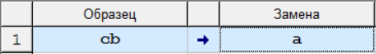
\includegraphics[width=.5\textwidth]{commands.png}
	\caption{Правила підстановки}
\end{figure}

\subsection*{Результат виконання програми}

\begin{figure}[h]
	\begin{subfigure}{.5\textwidth}
		\centering
		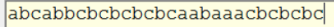
\includegraphics[width=.8\textwidth]{in.png}
		\subcaption{Вхідні дані}
	\end{subfigure}
	\hfill
	\begin{subfigure}{.5\textwidth}
		\centering
		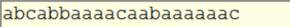
\includegraphics[width=.8\textwidth]{out.png}
		\subcaption{Вихідні дані}
	\end{subfigure}
	\caption{Демонстрація роботи програми}
\end{figure}

\section*{Висновок}

Виконуючи цю лабораторну робту, я ознайомився з принципами НАМ та навчився їх реалізовувати.

\section*{Відповіді на контрольні запитання}
\begin{itemize}
	\question З чого складається алгоритмічна система, заснована на відповідності
між словами в абстрактному алфавіті.
	\answer Алгоритмічна система, заснована на відповідності між словами в
		абстрактному алфавіті, включає об’єкти подвійної природи:
		\begin{enumerate}
				\item	Елементарні оператори --- алфавітні оператори за допомогою
					послідовного виконання яких реалізується будь-який алгоритм у даній
					алгоритмічній системі.
				\item	Елементарні розпізнавачі служать для розпізнавання присутності тих
					або інших властивостей інформації, яка переробляється алгоритмом, і для
					зміни, залежно від результатів розпізнавання, послідовності, в якій ідуть
					один за одним елементарні оператори.
		\end{enumerate}

	\question Що таке нормальний алгоритм Маркова?
	\answer Нормальним алгоритмом Маркова (НАМ) називається непорожній
скінчений впорядкований набір операторів підстановки.

	\question Правила виконання нормальних алгоритмів Маркова.
	\answer Робота НАМ зводиться до виконання послідовності кроків.
		На кожному кроці переглядаються зверху вниз оператори підстановки,
		що входять у НАМ і вибирається перший з операторів, який можна застосувати до вхідного слова р.
		Далі виконується підстановка відповідно до знайденого оператора. Отримуємо нове слово р1.

		На наступному кроці це слово р1 береться за початкове і до нього
		застосовується аналогічна процедура, тобто знову переглядаються зверху
		вниз оператори починаючи з самого верхнього і шукається перший
		оператор, який можна застосувати до слова р1, після чого виконується
		відповідна підстановка і отримується нове слово р2. І так далі.

	\question Як працює алгоритм, визначений граф-схемою?
	\answer вхідне слово подається на вхід і рухається у напрямках, які вказують стрілки. Коли слово попадає у вузол-розпізнавач, виконується перевірка умови, що в ньому задана. Якщо умова дотримана, слово прямує до операторного вузла, якщо ні — до наступного розпізнавача.

	\question Що таке узагальнені нормальні алгоритми?
	\answer Алгоритми, які задаються графами, складеними виключно з
розпізнавачів входження слів і операторів підстановки.

	\question У чому відмінність між УНА та НАМ?
	\answer Наявність у НАМ підстановок двох типів - завершальних і звичайних – є необхідною умовою універсальності НАМ, тобто можливості побудови НАМ, еквівалентного будь-якому наперед заданому алгоритму. Універсальність НАМ формулюється наступним принципом нормалізації. Для будь-якого алгоритму (алфавітного відображення, що конструктивно задається) у довільному скінченому алфавіті А можна побудувати еквівалентний йому нормальний алгоритм над алфавітом А.
\newpage
	\question Які способи композиції нормальних алгоритмів Вам відомі?
	\answer
	\begin{itemize}
		\item	cуперпозиція;
		\item	об'єднання;
		\item	розгалуження;
		\item	повторення.
	\end{itemize}
\end{itemize}

\end{document}
